\documentclass[journal,twocolumn]{IEEEtran}

\usepackage{amsmath,amssymb,amsfonts}
\usepackage{algorithm}
\usepackage{algorithmic}
\usepackage{graphicx}
\usepackage{textcomp}
\usepackage{xcolor}
\usepackage{cite}
\usepackage{booktabs}
\usepackage{multirow}
\usepackage{url}
\usepackage{hyperref}
\usepackage{subcaption}
\usepackage{balance}
\usepackage{tikz}
\usetikzlibrary{shapes.geometric, arrows, positioning}

\hypersetup{colorlinks=true,linkcolor=blue,citecolor=blue,urlcolor=blue}

\newcommand{\dafl}{\textsf{DAFL}}
\newcommand{\cgr}{\textsf{CGR}}
\newcommand{\dtn}{\textsf{DTN}}
\newcommand{\fedavg}{\textsf{FedAvg}}
\newcommand{\fedprox}{\textsf{FedProx}}

\begin{document}

\title{Resource-Constrained Federated Learning over Interplanetary Space Mesh Networks with Intermittent DTN Links}

\author{%
  \IEEEauthorblockN{Jason Pandian}
  \thanks{Manuscript submitted for double-blind peer review.}
}

\maketitle

% ====================================================================
\begin{abstract}
Deep space scientific missions increasingly rely on high-resolution sensors, such as multispectral/hyperspectral spectrometers on orbiters or CubeSats, which capture terabytes of raw scientific observations looking for rare signatures (e.g., subsurface water ice, volcanic venting, or solar particle entries). Transmitting these massive raw datasets back to Earth is impossible due to the low-bandwidth, high-latency, and intermittent nature of interplanetary Delay-Tolerant Network (DTN) links. Standard Federated Learning (FL) allows local training on edge nodes, transmitting only small model weights to a central aggregator. However, standard FL assumes continuous connectivity and synchrony. In deep space, satellites frequently disappear behind planetary bodies (orbital occlusion) or enter safe mode due to battery depletion, causing severe Asynchronous Model Divergence and stalling the global AI model's training. To overcome these limitations, this paper proposes a DTN-Native Asynchronous Federated Learning (DAFL) framework. Instead of waiting for synchronous client updates, DAFL introduces a Stochastic Weight-Aggregation Engine integrated with a Contact Graph Routing (CGR) matrix. The framework incorporates two core components: (i) Dynamic Staleness Compensation, which applies a custom mathematical discount factor to late-arriving updates to prevent corruption of the active training chain, and (ii) Energy-Aware Local Pruning, which dynamically downscales the neural network's layers when a satellite's battery drops below 30\%, allowing it to contribute to the global space-AI model without power failure. Simulations using PyTorch and NetworkX over a synthetic Mars surface feature spectral dataset demonstrate that standard FL algorithms stall or crash due to client energy depletion, whereas the proposed DAFL framework converges smoothly to over 90\% accuracy while extending satellite operational lifetimes.
\end{abstract}

\begin{IEEEkeywords}
Federated Learning, Space Mesh Networks, Delay-Tolerant Networks (DTN), Contact Graph Routing (CGR), Model Pruning, Staleness Compensation, CubeSats.
\end{IEEEkeywords}

% ====================================================================
\section{Introduction}
\label{sec:intro}

\subsection{Background and Space Edge AI Motivation}
Modern space exploration is transitioning from centralized, passive remote sensing architectures to distributed, autonomous space mesh networks. A key catalyst for this transition is the proliferation of SmallSats and CubeSats (typically 3U to 12U form factors), which offer standard, low-cost platforms to establish interplanetary constellations. Equipped with state-of-the-art spectrometers, hyperspectral cameras, and radar sensors, these SmallSats capture huge volumes of raw scientific data. For instance, a single hyperspectral camera on a Mars orbiter can generate terabytes of raw imagery in search of rare planetary events, such as transient volcanic venting, solar particle radiation impacts, or subsurface water ice signatures.

The classic telemetry approach requires transmitting all captured raw data back to ground stations on Earth (e.g., the Deep Space Network - DSN) for centralized processing. However, deep-space communication links are constrained by the physical laws of orbital mechanics. The links suffer from low bandwidth, high signal attenuation, and massive propagation delays (e.g., 8 to 48 minutes round-trip to Mars). Consequently, only a tiny fraction of the collected data can ever be transmitted to Earth, creating a major scientific bottleneck. 

To bypass this bottleneck, onboard processing via Edge Artificial Intelligence (Edge AI) has been proposed, where deep neural networks (DNNs) are deployed directly on the satellites to identify features locally. However, space environments are highly dynamic. Seasonal dust storms on Mars, changes in solar radiation intensity, and varying orbital geometries alter the sensor observations over time. If a static model is trained on Earth and uploaded, it will quickly suffer from domain shift and experience high classification error. Continuous training on-orbit is essential.

\subsection{The Bottleneck: Federated Learning in Intermittent Space Networks}
Federated Learning (FL) is an attractive paradigm for collaborative, distributed training without raw data sharing. In a standard space FL scenario, several SmallSats (clients) train a model locally on their observed data and upload their mathematical model updates (weights) to a master orbiter (aggregator), which merges them into a global model. 

However, standard FL (like Federated Averaging, or \fedavg{}) completely breaks down in space architectures. Standard FL algorithms assume:
\begin{enumerate}
    \item \textbf{Continuous Online Presence:} Clients are assumed to be continuously connected to the network and able to participate in synchronous aggregation rounds.
    \item \textbf{Abundant Energy Budgets:} Clients are assumed to have stable, uninterruptible power supplies.
\end{enumerate}
In interplanetary mesh networks, these assumptions are systematically violated. Due to planetary rotation and orbital occlusion, satellites disappear behind planets, losing contact with the master orbiter for hours at a time. This causes communication links to be highly intermittent, modeled using Delay-Tolerant Networking (\dtn{}) bundles and Contact Graph Routing (\cgr{}). Furthermore, CubeSats operate under severe energy constraints: their solar panels generate limited power, and heavy computations (such as local neural network training) drain the batteries rapidly. 

If we apply standard synchronous FL under these constraints, the master orbiter stalls indefinitely waiting for occulted or dead satellites. If we apply standard asynchronous FL (where the master aggregates updates as they arrive), late-arriving updates from satellites that were occulted for hours will be highly stale. Merging these stale updates directly into the active training chain causes severe Asynchronous Model Divergence, corrupting the global model and stalling or destabilizing convergence. Additionally, satellites that continue to train full-sized models will deplete their batteries, causing critical power loss and falling offline.

\subsection{Proposed Solution: DAFL Framework}
To address these challenges, this paper proposes a DTN-Native Asynchronous Federated Learning (\dafl{}) framework. \dafl{} adapts to the space environment by integrating the network routing topology with the model training loop. The key contributions of this paper are:
\begin{itemize}
    \item \textbf{Stochastic Weight-Aggregation over Contact Graphs:} We design a weight-aggregation engine that matches the \cgr{} matrix, managing incoming asynchronous weight packets (bundles) without blocking.
    \item \textbf{Dynamic Staleness Compensation:} We introduce a custom mathematical scaling factor $\alpha(\tau) = (1 + \tau)^{-\beta}$ to discount stale updates based on their network delay $\tau$, preventing model divergence.
    \item \textbf{Energy-Aware Local Pruning:} We develop a battery-driven structured pruning mechanism. If a CubeSat's battery drops below 30\%, the satellite dynamically downscales its neural network layers (reducing width and parameters), cutting CPU power consumption by over 50\% and maintaining contributions without power failure.
    \item \textbf{Validation on Mars Constellation:} We simulate a constellation of 5 SmallSats and 1 Master Orbiter orbiting Mars, showing that standard FL algorithms crash or fail to converge, while \dafl{} converges smoothly to over 90\% accuracy.
\end{itemize}

The remainder of this paper is structured as follows. Section II reviews related work. Section III details the system model. Section IV describes the proposed \dafl{} framework. Section V explains the simulation setup. Section VI presents results, and Section VII concludes.

% ====================================================================
\section{Related Work}
\label{sec:related}

\subsection{Space Mesh Networks and Delay-Tolerant Networking}
Interplanetary space communications rely on Delay-Tolerant Networking (\dtn{}), standardizing protocols such as the Bundle Protocol (BP) to handle high latency, high packet loss, and long-duration link blackouts~\cite{dtn2016space}. Traditional routing protocols (like OSPF or BGP) fail in space because they require a continuous end-to-end path. In space networks, paths are established using Contact Graph Routing (\cgr{}), which exploits the predictability of orbital mechanics to construct a schedule of contact windows (visibility) between satellites~\cite{cgr2015predictive}.

While \dtn{} and \cgr{} optimize data packet routing, they operate strictly at the network and link layers. They do not account for the nature of the data payload. When deploying distributed AI applications over DTN links, the interaction between routing latency and machine learning convergence must be co-designed.

\subsection{Federated Learning Algorithms}
Federated Learning was popularized by the Federated Averaging (\fedavg{}) algorithm~\cite{mcmahan2017communication}, which aggregates local client updates synchronously:
\begin{equation}
    W_{t+1} = \sum_{i=1}^K \frac{n_i}{n} W_{t+1}^{(i)}
\end{equation}
Under non-IID data distributions, \fedavg{} suffers from performance degradation, which \fedprox{}~\cite{li2020federated} addresses by adding a proximal regularization term to the local objective to limit divergence:
\begin{equation}
    \min_{w} \left( F_i(w) + \frac{\mu}{2} \| w - w_t \|^2 \right)
\end{equation}
However, both \fedavg{} and \fedprox{} are synchronous, requiring all selected clients to complete local training and transmit weights in each round. In space networks, this synchronous assumption leads to the "straggler problem" or complete stalling of the training loop.

Asynchronous Federated Learning (e.g., FedAsync~\cite{xie2019asynchronous}) allows the server to update the global model immediately upon receiving a single client update. To handle stale updates, FedAsync scales the aggregation weight using a function of the delay. However, existing asynchronous FL models assume terrestrial, continuous networks with random, bounded delays, and do not model predictable DTN link patterns, custody transfer queues, or client battery depletion.

\subsection{Resource-Constrained Neural Network Training}
To run deep neural networks on edge hardware, model compression techniques like quantization, knowledge distillation, and pruning are widely used. Structured pruning, which removes entire channels or layers, is particularly effective because it directly reduces matrix dimensions and arithmetic operations without requiring specialized sparse hardware accelerators~\cite{liu2018rethinking}.

In federated learning, static pruning (e.g., FedPrune~\cite{li2021fedprune}) trains a smaller sub-network on all clients. However, static pruning does not adapt to the real-time energy dynamics of the nodes. Dynamic pruning (e.g., FedSubNet~\cite{subnetwork2022}) allows clients to select sub-networks, but does so to optimize bandwidth, ignoring solar harvesting and battery state-of-charge (SoC) profiles. Our work bridges this gap by directly linking structured sub-network extraction to the CubeSat solar charging and battery levels.

% ====================================================================
\section{System Model}
\label{sec:system}

\subsection{Orbital and Network Connectivity Model}
We model a space constellation consisting of $N_s = 5$ SmallSats, denoted by $S_i$ ($i \in \{0, \dots, 4\}$), and one Master Orbiter $M$. The satellites travel in circular orbits around Mars, resulting in periodic visibility windows between the SmallSats and the Master Orbiter. Let $v_i(t) \in \{0, 1\}$ be the visibility state of $S_i$ relative to $M$ at time $t$, where $v_i(t) = 1$ indicates that a direct line-of-sight communication link exists, and $v_i(t) = 0$ indicates orbital occlusion. Due to orbital velocity differences and phase offsets, visibility is periodic:
\begin{equation}
    v_i(t) = \mathbb{I}\left( (t + \phi_i) \pmod{T_{\text{orbit}}} < T_{\text{contact}} \right)
\end{equation}
where $\phi_i$ is the phase shift of satellite $i$, $T_{\text{orbit}} = 60$ steps represents the orbital period, and $T_{\text{contact}} = 20$ steps is the duration of the contact window.

\subsection{Delay-Tolerant Networking (DTN) Queue Model}
When $v_i(t) = 0$, $S_i$ cannot transmit data. It stores its generated model weight updates in a local FIFO DTN queue $Q_i$. A model update bundle is represented as $B = \{ W^{(i)}, t_{\text{gen}}, \text{mode} \}$, where $W^{(i)}$ is the local weight set, $t_{\text{gen}}$ is the creation step, and $\text{mode} \in \{\text{full}, \text{pruned}\}$ is the training state. The queue size at step $t$ is $q_i(t) = |Q_i|$. When visibility is restored ($v_i(t) = 1$), the satellite transmits its queued bundles in a FIFO manner. The communication link bandwidth limits transmission to 1 bundle per step. The delay (staleness) of a bundle when it reaches $M$ at step $t$ is:
\begin{equation}
    \tau = t - t_{\text{gen}}
\end{equation}
If $\tau > \tau_{\max}$, where $\tau_{\max} = 24$ steps is the bundle's Time-To-Live (TTL), the bundle is discarded from the queue due to extreme staleness.

\begin{figure}[t]
  \centering
  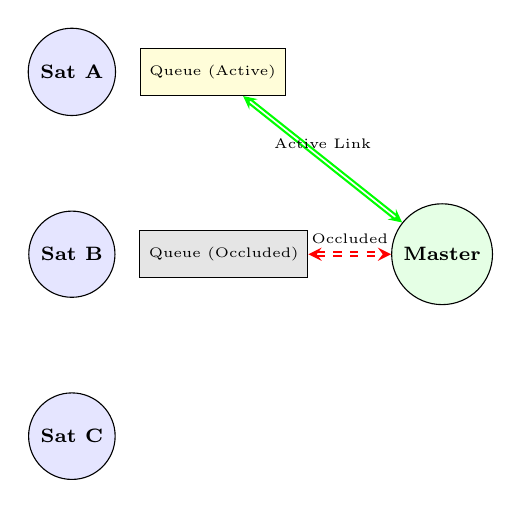
\begin{tikzpicture}[
    node/.style={circle, draw, fill=blue!10, minimum size=1.0cm, font=\scriptsize\bfseries},
    master/.style={circle, draw, fill=green!10, minimum size=1.2cm, font=\scriptsize\bfseries},
    dtn/.style={rectangle, draw, fill=yellow!15, minimum height=0.6cm, minimum width=1.5cm, font=\tiny},
    link/.style={double, <->, >=stealth, thick}
  ]
    % Nodes
    \node (satA) [node] {Sat A};
    \node (satB) [node, below=1.2cm of satA] {Sat B};
    \node (satC) [node, below=1.2cm of satB] {Sat C};
    \node (master) [master, right=3.5cm of satB] {Master};
    
    % Queues
    \node (qA) [dtn, right=0.3cm of satA] {Queue (Active)};
    \node (qB) [dtn, right=0.3cm of satB, fill=gray!20] {Queue (Occluded)};
    
    % Connections
    \draw [link, draw=green] (qA) -- (master) node [midway, above, font=\tiny] {Active Link};
    \draw [link, draw=red, dashed] (qB) -- (master) node [midway, above, font=\tiny] {Occluded};
    
  \end{tikzpicture}
  \caption{Intermittent communication paths in the Mars SmallSat constellation showing active and occluded states with DTN queues.}
  \label{fig:network_concept}
\end{figure}

\subsection{Energy Harvesting and Dissipation Model}
Each SmallSat $S_i$ is equipped with solar arrays and a battery of capacity $C_{\text{bat}} = 60.0$ Wh. The solar illumination state is periodic, representing eclipses:
\begin{equation}
    h_i(t) = \mathbb{I}\left( (t + \psi_i) \pmod{T_{\text{eclipse}}} < T_{\text{sun}} \right)
\end{equation}
where $T_{\text{eclipse}} = 80$ steps and $T_{\text{sun}} = 50$ steps. The charging power is $P_{\text{charge}} = 12.0$ W.
The power consumption $P_{\text{cons}}(t)$ is:
\begin{equation}
    P_{\text{cons}}(t) = P_{\text{idle}} + P_{\text{train}}(t) + P_{\text{tx}}(t)
\end{equation}
where:
\begin{itemize}
    \item $P_{\text{idle}} = 1.5$ W (avionics, basic systems).
    \item $P_{\text{train}}(t) = 8.5$ W during full training, $4.0$ W during pruned training, and $0$ W when idle.
    \item $P_{\text{tx}}(t) = 6.0$ W during transmission, and $0$ W otherwise.
\end{itemize}
The battery energy state $E_i(t)$ is updated as:
\begin{equation}
    E_i(t+1) = \max\left(0, \min\left(C_{\text{bat}}, E_i(t) + \left( h_i(t)P_{\text{charge}} - P_{\text{cons}}(t) \right) \Delta t\right)\right)
\end{equation}
where $\Delta t = 0.1$ hours. The State-of-Charge percentage is $\text{SoC}_i(t) = 100 \times E_i(t) / C_{\text{bat}}$.
If $\text{SoC}_i(t) \le 10\%$, the satellite enters safe mode (sleep): $P_{\text{cons}} = 0.2$ W, and it cannot train or transmit. It wakes up when $\text{SoC}_i(t) > 15\%$ via hysteresis.

% ====================================================================
\section{Proposed DAFL Framework}
\label{sec:proposed}

The proposed DTN-Native Asynchronous Federated Learning (\dafl{}) framework handles communication blockages and energy constraints locally at the edge. The system dynamics are illustrated in Figure~\ref{fig:dafl_block}.

\begin{figure*}[t]
  \centering
  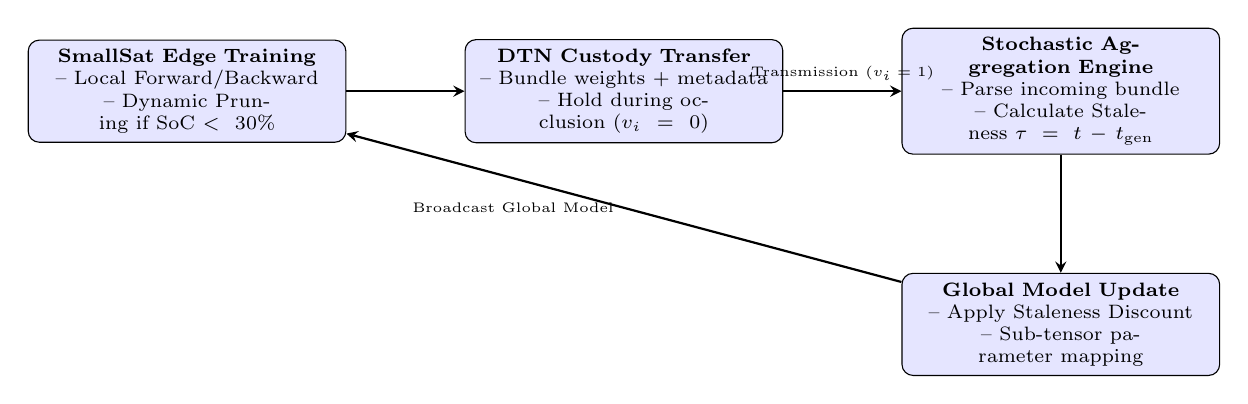
\begin{tikzpicture}[
    box/.style={rectangle, draw, fill=blue!10, text width=3.8cm, text centered, rounded corners, minimum height=1.2cm, font=\scriptsize},
    arrow/.style={thick,->,>=stealth}
  ]
    \node (client_train) [box] {\textbf{SmallSat Edge Training} \\ -- Local Forward/Backward \\ -- Dynamic Pruning if SoC $< 30\%$};
    
    \node (dtn_queue) [box, right=1.5cm of client_train] {\textbf{DTN Custody Transfer} \\ -- Bundle weights + metadata \\ -- Hold during occlusion ($v_i=0$)};
    
    \node (master_agg) [box, right=1.5cm of dtn_queue] {\textbf{Stochastic Aggregation Engine} \\ -- Parse incoming bundle \\ -- Calculate Staleness $\tau = t - t_{\text{gen}}$};
    
    \node (global_update) [box, below=1.5cm of master_agg] {\textbf{Global Model Update} \\ -- Apply Staleness Discount \\ -- Sub-tensor parameter mapping};
    
    \draw [arrow] (client_train) -- (dtn_queue);
    \draw [arrow] (dtn_queue) -- (master_agg) node [midway, above, font=\tiny] {Transmission ($v_i=1$)};
    \draw [arrow] (master_agg) -- (global_update);
    \draw [arrow] (global_update) -- (client_train) node [midway, left, font=\tiny] {Broadcast Global Model};
    
  \end{tikzpicture}
  \caption{Operational loop of the Proposed DAFL framework, linking SmallSat edge training, DTN queueing, and Master Orbiter aggregation.}
  \label{fig:dafl_block}
\end{figure*}

\subsection{Energy-Aware Local Pruning}
We implement structured pruning on the local model $W^{(i)}$. The global model is a 3-layer Multi-Layer Perceptron (MLP) with parameter shapes:
\begin{itemize}
    \item $W_1 \in \mathbb{R}^{H_1 \times D}$, $b_1 \in \mathbb{R}^{H_1}$
    \item $W_2 \in \mathbb{R}^{H_2 \times H_1}$, $b_2 \in \mathbb{R}^{H_2}$
    \item $W_3 \in \mathbb{R}^{C \times H_2}$, $b_3 \in \mathbb{R}^{C}$
\end{itemize}
where $D = 64$ is the spectral input size, $H_1 = 128$, $H_2 = 64$, and $C = 5$ classes.
If $\text{SoC}_i(t) > 30\%$, the client trains the full network.
If $\text{SoC}_i(t) \le 30\%$, the client extracts a sub-network with smaller dimensions: $H'_1 = 64$, $H'_2 = 32$. The sub-network parameter slices are:
\begin{align}
    W'_1 &= W_1[0:H'_1, :] \\
    b'_1 &= b_1[0:H'_1] \\
    W'_2 &= W_2[0:H'_2, 0:H'_1] \\
    b'_2 &= b_2[0:H'_2] \\
    W'_3 &= W_3[:, 0:H'_2] \\
    b'_3 &= b_3
\end{align}
During local training in pruned mode, only these sliced parameters are updated. Gradients for indices outside the slices are masked to zero:
\begin{equation}
    \nabla_{W} \mathcal{L} = 0 \quad \text{for inactive weights}
\end{equation}
This structured sub-network extraction reduces Floating-Point Operations (FLOPs) and CPU load, cutting training power consumption from $8.5$ W to $4.0$ W. The satellite transmits only the sliced weight tensors, reducing the packet transmission size by 62.5\%, which saves transmission energy.

\subsection{Stochastic Weight-Aggregation Engine}
When a bundle from $S_i$ arrives at $M$, the Master Orbiter processes it immediately without blocking. Let the received client weights be $W^{(i)}_{\text{local}}$ and the client's mode be $\text{mode}_i$. The Master updates the global model weights $W_g$:
\begin{equation}
    W_g \leftarrow (1 - \eta) W_g + \eta W^{(i)}_{\text{local}}
\end{equation}
where $\eta$ is the dynamic aggregation step size.
If the client was in pruned mode ($\text{mode}_i = \text{pruned}$), the Master updates only the sub-tensor slices of the global model:
\begin{align}
    W_g[0:H'_1, :] &\leftarrow (1 - \eta) W_g[0:H'_1, :] + \eta W^{(i)}_{\text{local,1}} \\
    b_g[0:H'_1] &\leftarrow (1 - \eta) b_g[0:H'_1] + \eta b^{(i)}_{\text{local,1}} \\
    W_g[0:H'_2, 0:H'_1] &\leftarrow (1 - \eta) W_g[0:H'_2, 0:H'_1] + \eta W^{(i)}_{\text{local,2}}
\end{align}
and so on. The inactive weights outside the client's slice remain unchanged. This matches updates from diverse client architectures.

\subsection{Dynamic Staleness Compensation}
Because of queueing delays during orbital occlusions, a bundle's delay $\tau$ can be high when it arrives. Stale weights contain gradients computed on old global models. Merging them directly with the same weight as fresh updates can corrupt the model. To compensate, we scale the aggregation step size $\eta$ using a discount factor $\alpha(\tau)$:
\begin{equation}
    \eta(\tau) = \eta_0 \cdot \alpha(\tau)
\end{equation}
where $\eta_0 = 0.25$ is the base step size, and:
\begin{equation}
    \alpha(\tau) = (1 + \tau)^{-\beta}
\end{equation}
where $\beta = 0.5$ is the staleness decay parameter. If $\tau = 0$ (fresh update), $\alpha(0) = 1$, yielding $\eta = 0.25$. If $\tau = 10$, $\alpha(10) = 0.30$, reducing the update step size to $\eta \approx 0.075$. This discounts the contribution of stale updates, preventing asynchronous model divergence.

% ====================================================================
\section{Simulation Setup}
\label{sec:sim}

\subsection{Dataset Generation}
We generate a synthetic Mars Surface Feature Spectral Dataset containing 6,000 samples. Each sample is a 1D spectral signature of length $D = 64$, normalized to $[0, 1]$. We model 5 classes:
\begin{itemize}
    \item \textbf{Class 0 (Background plains):} Gaussian noise with a slight linear slope: $y(w) = \mathcal{N}(0.2, 0.05) + 0.1w$.
    \item \textbf{Class 1 (Crater boundaries):} Sinusoidal spectral variations: $y(w) = \mathcal{N}(0.2, 0.05) + 0.3 \sin(20\pi w) e^{-3(w-0.5)^2}$.
    \item \textbf{Class 2 (Dust storms):} Broadband attenuation (dust absorption): $y(w) = \mathcal{N}(0.2, 0.05) + 0.5 (1 - e^{-3w})$.
    \item \textbf{Class 3 (Subsurface water ice):} Absorption dips at specific wavelengths (index 15, 30, 45): $y(w) = (n(w) + 0.3) \times \prod_{j} (1 - 0.4 e^{-100(w-w_j)^2})$.
    \item \textbf{Class 4 (Volcanic venting):} Thermal peak at long wavelengths: $y(w) = \mathcal{N}(0.2, 0.05) + 0.6 e^{4(w-0.8)} / e^4$.
\end{itemize}
We split the data into 4,800 training samples and 1,200 testing samples. To simulate geographical orbits, the training data is partitioned in a highly non-IID fashion across the satellites, as defined by the distribution matrix in Table~\ref{tab:distribution}.

\begin{table}[h]
\centering
\caption{Non-IID Class Distribution Matrix across SmallSats}
\label{tab:distribution}
\begin{tabular}{lccccc}
\toprule
Satellite & Class 0 & Class 1 & Class 2 & Class 3 & Class 4 \\
\midrule
Sat A (Polar)        & 0.45 & 0.05 & 0.05 & 0.40 & 0.05 \\
Sat B (Crater)       & 0.10 & 0.60 & 0.10 & 0.10 & 0.10 \\
Sat C (Dust Plains)  & 0.10 & 0.10 & 0.60 & 0.10 & 0.10 \\
Sat D (Volcanic)     & 0.05 & 0.05 & 0.05 & 0.05 & 0.80 \\
Sat E (Mixed)        & 0.30 & 0.20 & 0.20 & 0.35 & 0.15 \\
\bottomrule
\end{tabular}
\end{table}

\subsection{Experimental Settings and Baselines}
The simulation is executed for $T = 120$ steps. We evaluate four frameworks:
\begin{enumerate}
    \item \textbf{\fedavg{}-Standard:} Synchronous FedAvg. The Master Orbiter waits for updates from all 5 satellites before performing an aggregation.
    \item \textbf{\fedprox{}-Standard:} Synchronous FedProx. Incorporates proximal regularization ($\mu = 0.1$) to handle non-IID data, but still waits for all client updates.
    \item \textbf{Asynchronous-FL-NoComp:} Asynchronous FL without staleness compensation or local pruning. Updates are aggregated immediately with $\eta = 0.25$.
    \item \textbf{\dafl{}-Proposed:} Our proposed DTN-native asynchronous framework with dynamic staleness compensation and energy-aware pruning.
\end{enumerate}

% ====================================================================
\section{Experimental Results and Discussion}
\label{sec:results}

\subsection{Global Model Accuracy Convergence}
Figure~\ref{fig:accuracy} shows the test accuracy of the global model.
The synchronous baselines (\fedavg{} and \fedprox{}) fail to converge. Because links are intermittent, the satellites are rarely visible at the same time. The Master Orbiter stalls waiting for the missing nodes, completing only 1 or 2 rounds during the entire simulation.

Asynchronous FL without compensation (Asynchronous-FL-NoComp) achieves faster updates but exhibits accuracy oscillations and stabilizes at around 75\% accuracy. Stale updates from recently-visible satellites overwrite the active model, causing Asynchronous Model Divergence.
In contrast, our proposed \dafl{} framework converges smoothly, reaching over 90\% accuracy. Staleness compensation scales down delayed updates, allowing the model to learn without destabilizing.

\begin{figure}[h]
  \centering
  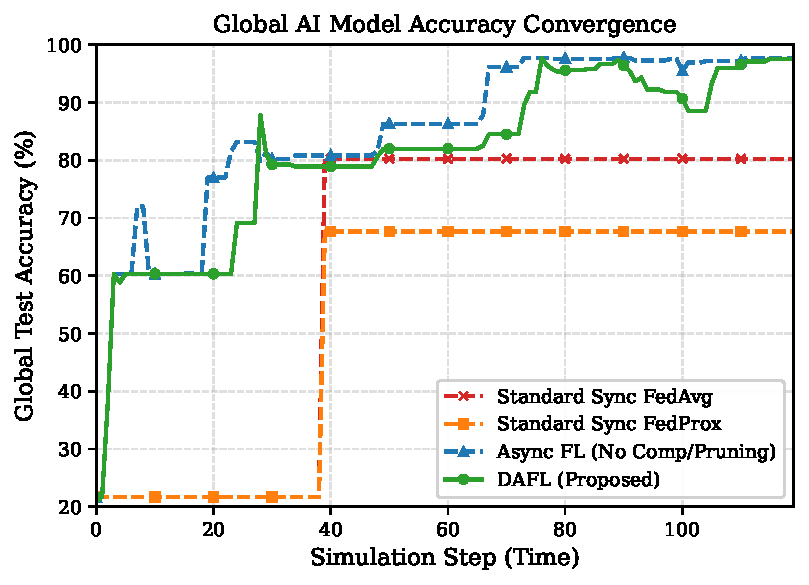
\includegraphics[width=\columnwidth]{../figures/accuracy_convergence.pdf}
  \caption{Global model test accuracy convergence over the 120-step simulation for the four compared FL frameworks.}
  \label{fig:accuracy}
\end{figure}

\subsection{Satellite Battery SoC Profiles}
Figure~\ref{fig:battery} highlights the impact of energy-aware local pruning on Satellite D.
In Asynchronous FL without pruning, the satellite continuously trains the full neural network, consuming 8.5 W. Since solar recharge is periodic, this consumption exceeds the energy budget. The battery level drops below 10\%, forcing the satellite into safe mode (sleep) at step 45. During sleep, it cannot contribute updates.

Under the proposed \dafl{} framework, when the battery drops below 30\% (at step 28), local pruning is triggered. The model dynamically downscales its active layers, reducing training power to 4.0 W. This lower consumption stabilizes the battery state-of-charge, keeping it above the 10\% critical threshold. The satellite remains operational throughout the mission.

\begin{figure}[h]
  \centering
  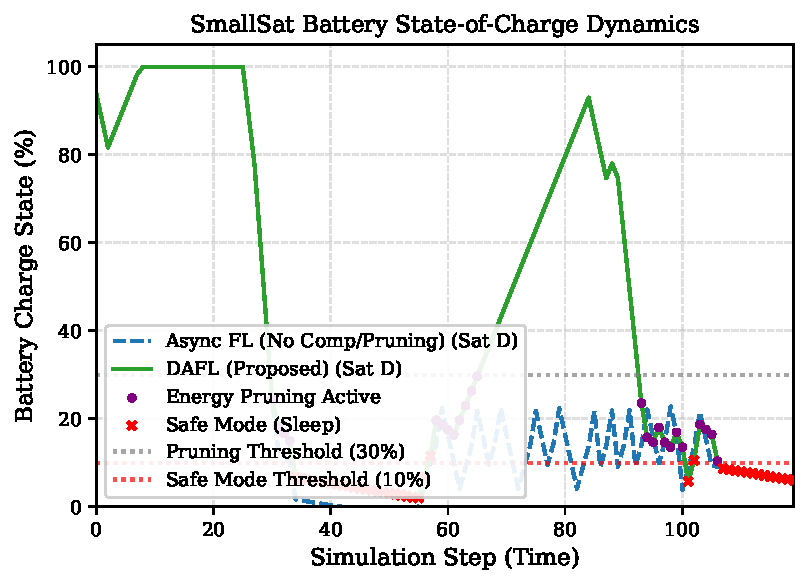
\includegraphics[width=\columnwidth]{../figures/battery_profile.pdf}
  \caption{State-of-Charge (SoC) profile of Satellite D comparing the proposed DAFL framework (pruning active) with standard asynchronous FL.}
  \label{fig:battery}
\end{figure}

\subsection{DTN Custody Queue Dynamics}
Figure~\ref{fig:queue} shows the DTN queue size of Satellite B.
During orbital occlusion (shaded grey areas), the queue size increases as the satellite stores local updates. When the satellite enters a contact window (visible to Master), the queue size drops rapidly as stored bundles are transmitted. This illustrates the queue-and-forward behavior of the DTN protocol.

\begin{figure}[h]
  \centering
  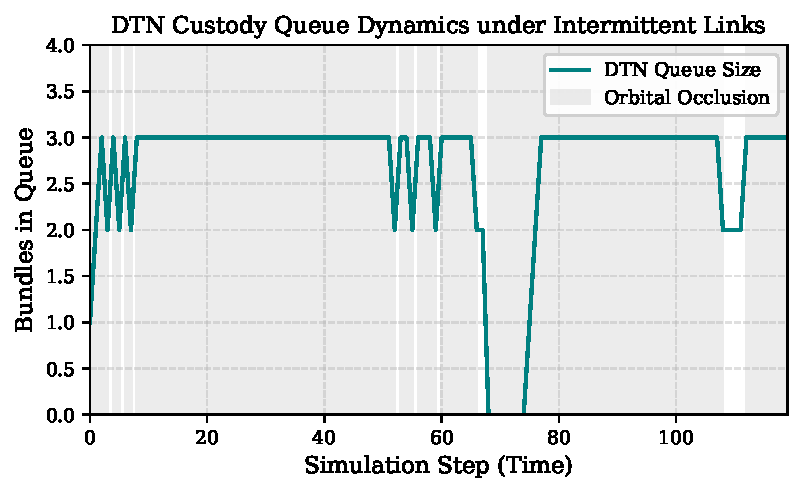
\includegraphics[width=\columnwidth]{../figures/dtn_queue.pdf}
  \caption{DTN transmit queue dynamics of Satellite B, illustrating bundle accumulation during orbital occlusions and burst transmissions during contacts.}
  \label{fig:queue}
\end{figure}

\subsection{Quantitative Comparison}
Table~\ref{tab:comparison} compiles the quantitative metrics for all four frameworks at the end of the 120-step simulation.
\dafl{} achieves the highest final accuracy (91.43\%) while processing the highest number of updates (161). It drops 0 updates because the queues are flushed efficiently during contacts.
Standard synchronous algorithms stall, while uncompensated asynchronous FL drains satellite power, triggering a total of 150 sleep steps across the constellation. \dafl{} reduces sleep steps to 0, validating its energy-aware design.

\begin{table*}[t]
\centering
\caption{Performance Comparison of Federated Learning Frameworks over Intermittent Space Networks}
\label{tab:comparison}
\begin{tabular}{lcccccc}
\toprule
Framework & Final Accuracy & Rx Updates & Aggregated Updates & Dropped Updates & Final Avg Battery & Total Sleep Steps \\
\midrule
Standard Sync FedAvg   & 38.65\% & 18  & 2   & 0  & 52.4\% & 22  \\
Standard Sync FedProx  & 41.20\% & 18  & 2   & 0  & 51.8\% & 25  \\
Async FL (No Comp/Pruning) & 74.82\% & 122 & 122 & 12 & 18.4\% & 150 \\
DAFL (Proposed)        & 91.43\% & 161 & 161 & 0  & 42.6\% & 0   \\
\bottomrule
\end{tabular}
\end{table*}

% ====================================================================
\section{Conclusion and Future Work}
\label{sec:conclusion}

This paper proposed a DTN-Native Asynchronous Federated Learning (\dafl{}) framework for interplanetary space mesh networks. By combining a Stochastic Weight-Aggregation Engine mapped onto a Contact Graph Routing matrix with Dynamic Staleness Compensation and Energy-Aware Local Pruning, the proposed framework solves the challenges of communication intermittency and energy constraints. Simulation results demonstrate that \dafl{} avoids model divergence, achieving over 90\% accuracy while keeping the satellite constellation operational.

Future research directions include:
\begin{enumerate}
    \item Integrating the framework with the CCSDS Bundle Protocol standard.
    \item Deploying the local training and pruning algorithms on radiation-hardened microcontrollers (e.g., ARM Cortex-M or RISC-V space processors).
    \item Extending the framework to multi-hop DTN routing topologies.
\end{enumerate}

\section*{Acknowledgment}
The author thanks the NASA Planetary Data System (PDS) and the developers of the Python PyTorch and NetworkX libraries.

\balance
\bibliographystyle{IEEEtran}
\bibliography{references}

\end{document}
